\subsection{Setup initial}
Toute cette partie est normalement couverte par *insérer nom du doc pour la création d'un site laravel en utilisant Docker Desktop*. Normalement, à la suite de tutoriel, vous devriez avoir obtenu le site suivant en vous rendant sur \url{http://jsp}:
\begin{figure}[!h]
    \centering
    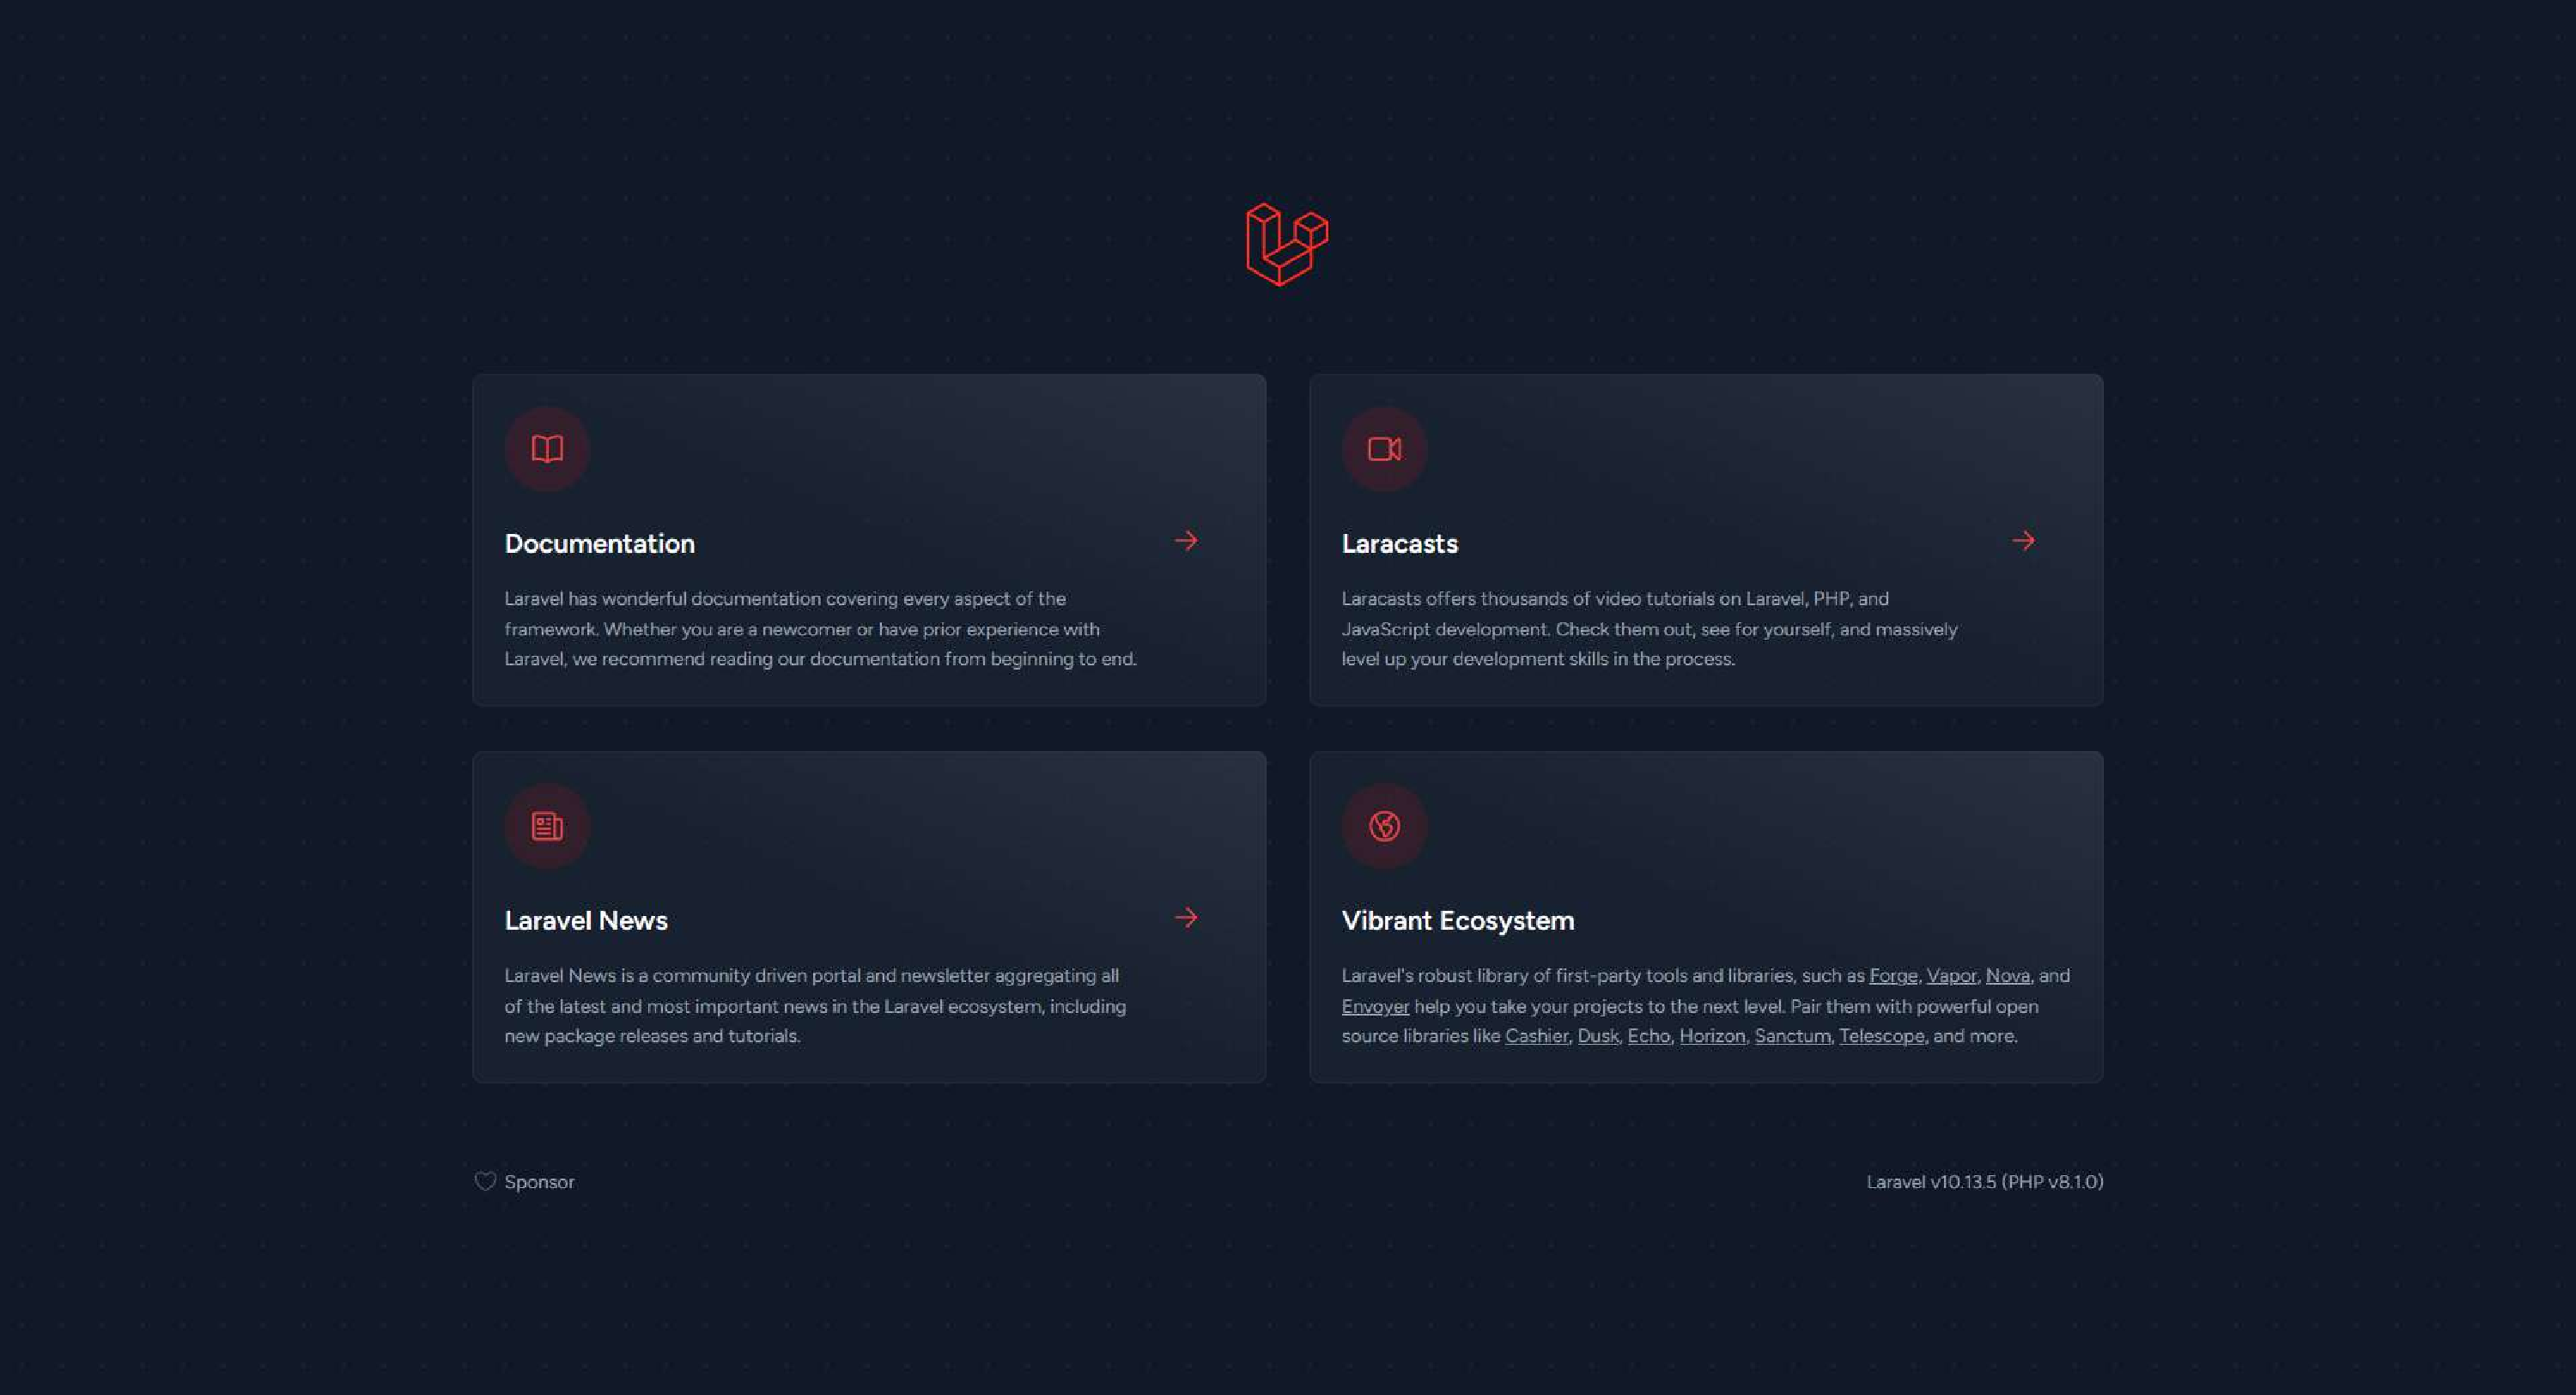
\includegraphics[width=0.75\textwidth]{figures-C1/laravel_default_website.pdf}
\end{figure}
Nous allons partir de ce site là. Pour ce tutoriel, mon projet sera appellé \texttt{tutorialstepbystep} donc son URL sera \url{http://tutorialstepbystep/}.
